%\documentclass[iop]{emulateapj}
\documentclass[aps, pre, onecolumn, nofootinbib, notitlepage, groupedaddress, amsfonts, amssymb, amsmath, longbibliography]{revtex4-1}
\usepackage{graphicx}
\usepackage{hyperref}
\usepackage{xcolor}
\usepackage{subcaption}
\hypersetup{
    colorlinks,
    linkcolor={red!50!black},
    citecolor={blue!50!black},
    urlcolor={blue!80!black}
}
\usepackage{bm}
\usepackage{natbib}
%\usepackage{longtable}
%\LTcapwidth=0.87\textwidth

\newcommand{\Div}[1]{\ensuremath{\nabla\cdot\left( #1\right)}}
\newcommand{\angles}[1]{\ensuremath{\left\langle #1 \right\rangle}}
\newcommand{\grad}{\ensuremath{\nabla}}
\newcommand{\RB}{Rayleigh-B\'{e}nard }
\newcommand{\stressT}{\ensuremath{\bm{\bar{\bar{\Pi}}}}}
\newcommand{\lilstressT}{\ensuremath{\bm{\bar{\bar{\sigma}}}}}
\newcommand{\nrho}{\ensuremath{n_{\rho}}}
\newcommand{\approptoinn}[2]{\mathrel{\vcenter{
	\offinterlineskip\halign{\hfil$##$\cr
	#1\propto\cr\noalign{\kern2pt}#1\sim\cr\noalign{\kern-2pt}}}}}

\newcommand{\appropto}{\mathpalette\approptoinn\relax}

\newcommand\mnras{{MNRAS}}%

\begin{document}
\title{BVPs to assist in convergence of Rayleigh-Benard systems}
\maketitle

\section{The Boussinesq equations}
Just to make sure I'm on the same page as anyone I send this to, the Boussinesq equations are
\begin{equation}
\begin{split}
&\Div{\bm{u}} = 0 \\
&\frac{\partial \bm{u}}{\partial t} + \bm{u}\cdot\grad\bm{u} = -\grad P + T_1\hat{z} + \frac{\text{Pr}}{\text{Ra}}\grad^2 \bm{u} \\
&\frac{\partial T_1}{\partial t} + \bm{u}\cdot\grad T_1 + w\frac{\partial T_0}{\partial z} = \frac{1}{\text{Pr Ra}}\grad^2 T_1,
\end{split}
\end{equation}
where $\bm{u} = u\hat{x} + w\hat{z}$ is velocity (in 2D), $T_1$ is temperature fluctuations around the background, $T_0$, and then $P$ is our pressure but it's
really just a fancy thing that instantaneously enforces $\Div{\bm{u}} = 0$.  Ra is the Rayleigh number,
Pr is the Prandtl number, and these equations have been non-dimensionalized on the
free-fall time.

\section{The BVP equations}
The Boussinesq equations (and Rayleigh Benard convection) have something really nice
going for them that stratified convection doesn't: symmetry.  Upflows and downflows are
symmetric, so $\angles{w} = 0$, where $\angles{A} = \int A dx\,dt / (L_x T)$, where
$L_x$ is the horizontal width of the atmosphere and $T$ is the time over which the
average is taken.  This also means that $\angles{\partial w / \partial t} = 0$ (I think,
I have to check this to be certain because of the time in the integral).  And this
means that when you take the average of the momentum equation, all of the terms in
it have to add up to a zero horizontal average:
$$
\angles{\bm{u}\cdot\grad w + \grad P - T_1 - \frac{\text{Pr}}{\text{Ra}}\grad^2 w} = 0,
$$
and this also means that any BVP adjustments I solve for around the IVP need to satisfy
$$
\grad P_{\text{BVP}} - T_{\text{BVP}} = 0.
$$
So...hooray, $P$ is given to us for free.

If we look at the energy equation, we can acknowledge that (in Boussinesq),
$$
\bm{u}\cdot\grad A = \Div{\bm{u}A},
$$
and there's an extra $A\Div{\bm{u}}$ term on the RHS, but that's zero in this
approximation.  If we rearrange the energy equation, we get
$$
\frac{\partial T_1}{\partial t} + \Div{\bm{u} T_1 - \frac{1}{\text{Pr Ra}} \grad T_1} + w\frac{\partial T_0}{\partial z} = 0.
$$
If we take an average of this equation, we get
$$
\angles{\frac{\partial T_1}{\partial t} + \Div{\bm{u} T_1 - \frac{1}{\text{Pr Ra}} \grad T_1} + w\frac{\partial T_0}{\partial z}} = 0.
$$
Now, basically what we're doing in this BVP method is saying that we want the time-stationary state, such that $\angles{\partial T_1/\partial z} = 0$.
The last term on the RHS is $\angles{ w \partial_z T_0} = \angles{w}\partial_z T_0 = 0$ by symmetry.
We also assume that $T_1 \equiv T_1 + T_{\text{BVP}}$, where $T_1$ is from the IVP,
and $T_{\text{BVP}}$ is from the BVP.
The full remaining equation here is then
$$
\angles{\partial_x \left( u (T_1 + T_{\text{BVP}}) - \frac{1}{\text{Pr Ra}} \partial_x (T_1 + T_{\text{BVP}}) \right)}
+ \angles{\partial_z \left( w (T_1 + T_{\text{BVP}}) - \frac{1}{\text{Pr Ra}} \partial_z (T_1 + T_{\text{BVP}} \right)} = 0
$$
In these systems on fourier bases, over long timescales, we don't expect any horizontal average of the
horizontal flux's divergence.  Furthermore, the BVP contribution to the enthalpy flux
is $\angles{w T_{\text{BVP}}} = \angles{w} T_{\text{BVP}} = 0$.  Thus, we're left with
\begin{equation}
\frac{1}{\text{Pr Ra}}\frac{\partial^2 T_{\text{BVP}}}{\partial z^2} = 
\frac{\partial}{\partial z}\left( \angles{w T_1} - \frac{1}{\text{Pr Ra}} 
\frac{\partial}{\partial z}\angles{T_1}\right)
\end{equation}
Or, put a different way:
\begin{equation}
\frac{1}{\text{Pr Ra}}\frac{\partial^2 T_{\text{BVP}}}{\partial z^2} = 
\frac{\partial}{\partial z}\left( \text{(Enth IVP)} + \text{(Cond IVP)}\right)
\end{equation}
Where ``Enth IVP'' is the enthalpy flux from the IVP, and ``Cond IVP'' is the conductive
flux from the IVP.  What we're doing with this equation is adjusting the system's
conductive flux such that, on average, our system is in flux equilibrium.

\subsection{Subtleties}
In general, during the transient, the enthalpy flux is:
\begin{enumerate}
\item Too large (the transient velocities are higher than the converged velocities).
\item Asymmetric (the evolving temperature profile still has some bias from the initial
conditions, and the enthalpy flux feels that bias).
\end{enumerate}
Because of these two things, if we straight up solve the BVP equation from above, we'll end up
with a wonky adjustment to the temperature profile.  To make our system more smart about the
BVP, we can go through the following process:
\begin{enumerate}
\item Fit a line to the middle of the enthalpy flux profile.
\item Divide the enthalpy flux profile by that line (this flattens it out in the middle fairly well).
\item Multiply the profile such that all of the system flux is carried by enthalpy flux in the interior.
\item Use that new enthalpy flux profile while solving for the BVP.
\end{enumerate}
In doing so, we get close to the evolved temperature profile we want.  
For an example of this, see Figure \ref{fig:bvp_results}.

\begin{figure}[b!]
\begin{subfigure}{.5\textwidth}
\centering
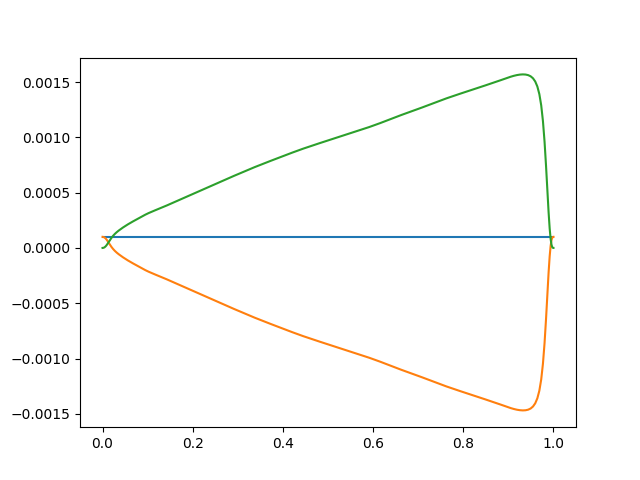
\includegraphics[width=.8\linewidth]{figs/fluxes_0000.png}
\caption{1a The enthalpy flux (green), radiative flux (orange), and total flux
(blue) of a BVP that directly uses IVP profiles as inputs}
\label{fig:sfig1}
\end{subfigure}%
\begin{subfigure}{.5\textwidth}
\centering
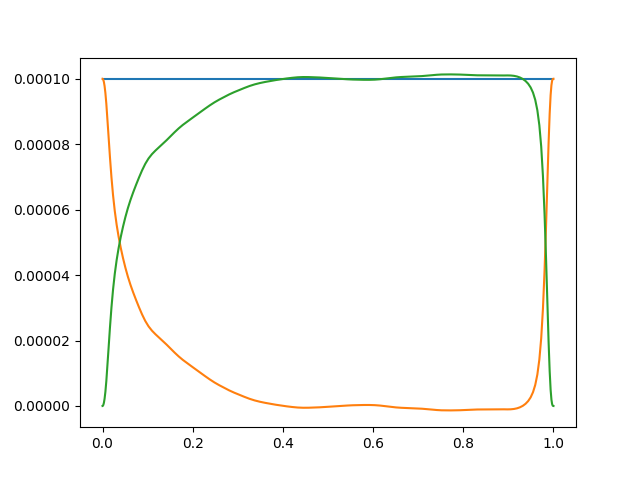
\includegraphics[width=.8\linewidth]{figs/fluxes_0001.png}
\caption{1a The enthalpy flux (green), radiative flux (orange), and total flux
(blue) of a BVP that uses a modified enthalpy flux as an input}
\end{subfigure}
\caption{Two plots of the adjusted flux profiles after a BVP is run. In
Fig. 1a, the time averaged profiles from the IVP are directly used in the BVP solve.
In Fig. 2a, the best-fit line to the mid-domain enthalpy flux is divided out of the enthalpy flux,
and then the profile is appropriately scaled.  The resulting temperature profile from the BVP is then
close to the desired evolved solution.}
\label{fig:bvp_results}
\end{figure}

\bibliography{../biblio.bib}
\end{document}
